% $Id: specifyTestCases.tex 8144 2009-04-03 15:27:38Z alexandra $
% Local Variables:
% ispell-check-comments: nil
% Local IspellDict: american
% End:
% --------------------------------------------------------
% User documentation
% copyright by BREDEX GmbH 2004
% -------------------------------------------------------
\index{New!Test Case}
\index{Test Case!New}

Most of the time spent writing tests will involve creating and editing \gdcases{}. 

To create a \gdcase{}, you must have created or opened a \gdproject{} \bxpref{WorkingWithProjects}. 

The \gdtestcasebrowser{} must also be visible. If it is not visible, change to the \specpersp{} perspective and select:\\
\bxmenu{Window}{Show View}{Test Case Browser}.

\begin{enumerate}
\item Create a \gdcase{} by using the context-sensitive menu in the \gdtestcasebrowser{}:\\
\bxmenu{New}{New \gdcase{}}{}.
\bxtipp{You can also create \gdcases{} with a double-click on the \bxcaption{\gdcases{}:} root entry or on a category in the \gdtestcasebrowser{}.}

\item A dialog to name the \gdcase{} will appear (\bxfigref{newtestcasedialog}). Because \app{} is keyword-driven, it is important to name \gdcases{} meaningfully --  you will be able to read your tests easily and quickly choose which \gdcase{} you need  \bxpref{BPTestCaseNames}. 

\begin{figure}[h]
\begin{center}
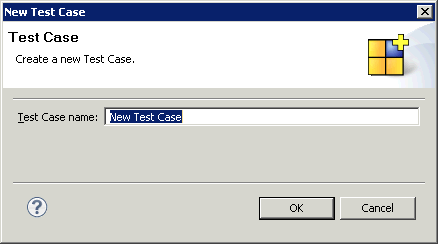
\includegraphics[width=12.5cm]{Tasks/Testcases/PS/newtestcasedialog}
\caption{New \gdcase{} Dialog}
\label{newtestcasedialog}
\end{center}
\end{figure} 

\item Click \bxcaption{OK}. 
\item This creates a new \gdcase{} with that name in the \gdtestcasebrowser{} \bxfigref{newtestcaseinbrowser}.

\begin{figure}[h]
\begin{center}
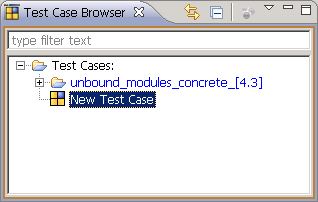
\includegraphics{Tasks/Testcases/PS/newtestcaseinbrowser}
\caption{\gdcase{} in \gdtestcasebrowser{}}
\label{newtestcaseinbrowser}
\end{center}
\end{figure} 

\end{enumerate}

\bxtipp{See the Best Practices section for information on how to best structure your \gdcases{} and tests \bxpref{BPKeywordDesign}.}
\textbf{Next steps}\\
The next step is to add \gdcases{} from the library of \gdcases{} to this \gdcase{}\bxpref{usingtemplate}. 

You can also:
\begin{itemize} 
\item Reuse this \gdcase{} to form other \gdcases{}  \bxpref{TasksEditorAdd}
\item Edit its content in the \gdtestcaseeditor{} \bxpref{WorkingWithEditors}
\item Add this \gdcase{} to a \gdsuite{} to be executed \bxpref{TasksEditorAdd}
\item Use this \gdcase{} as an \gdehandler \bxpref{customizedehandler}. 
\end{itemize}













